\section{První verze}
\label{M1-vyvoj}

\begin{wrapfigure}{R}[20mm]{0.4\textwidth}
    \centering
    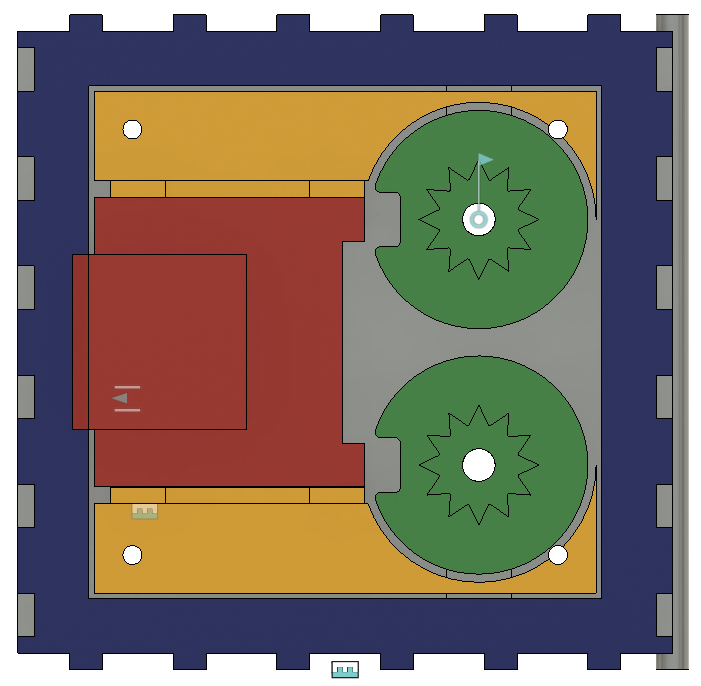
\includegraphics[width=0.4\textwidth]{kapitoly/obrazky/M1/mechanizmus.png}
    \caption{Zelená barva značí kódovací kola, červená západku, modrá pevnou část trezoru a žluté díly distanci \centering}
    \label{fig:M1-mechanizmus}
\end{wrapfigure}
První čistě mechanická varianta, označovaná jako M1, vznikla začátkem srpna 2019, brzy po první  elektronické variantě.
Měla stále poměrně klasický vzhled trezoru -- zamykatelná skříňka se dvěma  kódovacími koly, která ovládala možnost pohybu jednoduché západky.

Tato verze byla také určená jako základ pro plánovaný upgrade na další elektronickou
variantu. Na podobné vylepšení mělo stačit odstranění kódo\-va\-cích kol a přidělání elektronické části. Toto sice fungovalo obstojně, zároveň 
i~jako motivace, ale kvůli pozdější změně konceptu mechanizmu uzavírání trezoru\footnote{místo rotační západky mechanizmus bajonetu -- viz kapitola %todo
} tento nápad padl.

Tato varianta se také ukázala jako nevhodná\footnote{kvůli přílišné náročnosti na přesnost sesazení} pro stavbu s malými dětmi, 
pro které byla určena jakožto předstupeň k variantě elektronické (která vyžaduje i~znalosti programování nebo alespoň ochotu se jej  učit).